% !TeX program = xelatex
\RequirePackage{fix-cm}
\documentclass[14pt,a4paper]{extarticle}
\usepackage{fontspec}
\defaultfontfeatures{Ligatures=TeX}
\input{build/font-path.tex}
\ifdefined\reportFontPath
  \setmainfont{Times.TTF}[Path=\reportFontPath,BoldFont=Timesbd.TTF,ItalicFont=Timesi.TTF,BoldItalicFont=Timesbi.TTF]
  \newfontfamily\cyrillicfont{Times.TTF}[Path=\reportFontPath,BoldFont=Timesbd.TTF,ItalicFont=Timesi.TTF,BoldItalicFont=Timesbi.TTF,Script=Default]
\else
  \setmainfont{Times New Roman}
  \newfontfamily\cyrillicfont{Times New Roman}
\fi
\setmonofont{FreeMono}
\newfontfamily\cyrillicfonttt{FreeMono}
\usepackage{polyglossia}
\setdefaultlanguage{russian}
\setotherlanguage{english}
\usepackage[left=30mm,right=10mm,top=20mm,bottom=20mm,footskip=10mm]{geometry}
\usepackage{setspace}
\makeatletter
\renewcommand{\normalsize}{\@setfontsize\normalsize{14bp}{16.8bp}}
\makeatother
\onehalfspacing
\AtBeginDocument{\normalsize}
\setlength{\parindent}{1.25cm}
\setlength{\parskip}{0pt}
\usepackage{indentfirst}
\usepackage{array,tabularx,graphicx,float,caption,fvextra}
\DeclareCaptionLabelSeparator{gost}{~—~}
\captionsetup{font=small,labelsep=gost,justification=centering,singlelinecheck=false}
\captionsetup[table]{justification=raggedright,position=top,skip=6pt}
\captionsetup[figure]{skip=8pt}
\addto\captionsrussian{\renewcommand{\figurename}{Рисунок}\renewcommand{\tablename}{Таблица}}
\usepackage{titlesec}
\titleformat{\section}[block]{\normalfont\bfseries\centering}{\thesection.}{.5em}{\MakeUppercase}
\titlespacing*{\section}{0pt}{0pt}{18pt}
\usepackage{enumitem}
\usepackage{xurl}
\urlstyle{same}
\usepackage[hidelinks,unicode,pdfauthor={Матвеев М. А.},pdftitle={Лабораторная работа №7. Адаптивная вёрстка и медиазапросы}]{hyperref}
\pagestyle{plain}
\emergencystretch=2em
\clubpenalty=10000
\widowpenalty=10000
\raggedbottom
\newcolumntype{Y}{>{\raggedright\arraybackslash}X}
\newcommand{\code}[1]{{\fontsize{12}{14}\selectfont\texttt{#1}}}
\newcommand{\listing}[1]{\begingroup\singlespacing\VerbatimInput[breaklines=true,breakanywhere=true,fontsize=\fontsize{9.5}{11.5}\selectfont,numbers=left,numbersep=6pt,xleftmargin=16pt]{#1}\endgroup}

\begin{document}
\begin{titlepage}
\thispagestyle{empty}
\begin{center}
\bfseries
МИНОБРНАУКИ РОССИИ\\
Федеральное государственное автономное\\
образовательное учреждение высшего образования\\
«Санкт-Петербургский государственный\\
электротехнический университет «ЛЭТИ»\\
им. В.И. Ульянова (Ленина)»\\
Кафедра информационных систем
\end{center}
\vspace{30mm}
\begin{center}
\textbf{ОТЧЕТ ПО ЛАБОРАТОРНОЙ РАБОТЕ №7}\\[8mm]
«Адаптивная вёрстка и медиазапросы»
\end{center}
\vfill
\noindent\begin{tabularx}{\textwidth}{@{}lXr@{}}
Студент гр. 4372 & \centering\rule{25mm}{0.3pt} & Матвеев М. А.\\[8mm]
Преподаватель & \centering\rule{25mm}{0.3pt} & Нечитайленко Р. А.\\
\end{tabularx}
\vspace{20mm}
\begin{center}
Санкт-Петербург\\
2026
\end{center}
\end{titlepage}
\setcounter{page}{2}

\section{Цель и выполнение работы}
Цель работы: изменить оформление страницы с помощью медиазапросов и построить адаптивную сетку карточек.

В \code{media.html} размещён отдельный пример смены цвета текста. При ширине окна до 480~px текст красный, от 481 до 800~px зелёный, свыше 800~px синий. Пороговые значения включаются в условия \code{max-width}.

Страница \code{index.html} содержит шесть карточек с иллюстрациями и абзацами. На широком экране сетка имеет три колонки, до 800~px две, до 480~px одну. Изображение взято из предоставленного образца: CSS ограничивает видимую область иллюстрацией, сохраняя исходный снимок без изменений.
\begin{figure}[H]
\centering
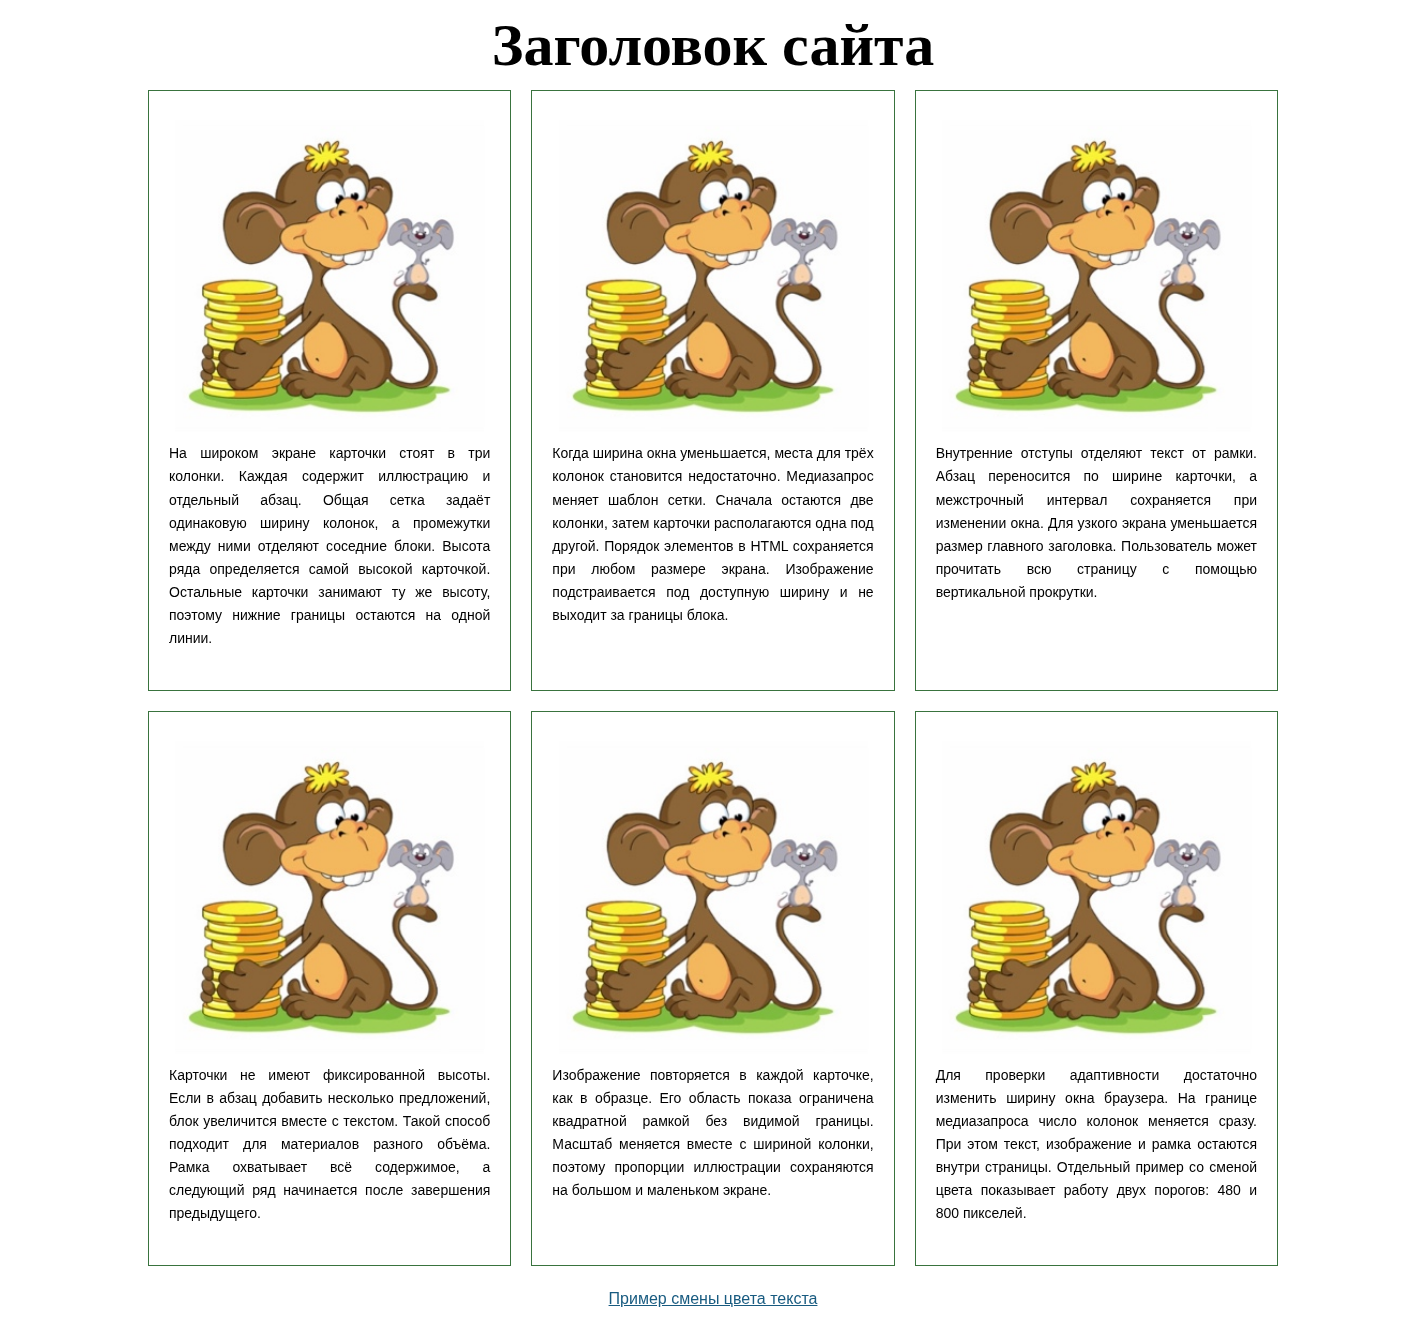
\includegraphics[width=\textwidth,height=150mm,keepaspectratio]{assets/desktop.png}
\caption{Сетка карточек при ширине окна 1426 px}
\end{figure}

\clearpage
\section{Проверка медиазапросов}
В Chromium 153 проверены значения непосредственно на границах медиазапросов и рядом с ними.
\begin{table}[H]
\caption{Проверка порогов медиазапросов}
\begingroup\fontsize{12}{14}\selectfont\singlespacing
\renewcommand{\arraystretch}{1.25}
\begin{tabularx}{\textwidth}{|Y|Y|Y|}
\hline
Ширина окна, px & Цвет текста & Число колонок\\ \hline
320 и 480 & Красный & 1\\ \hline
481 и 800 & Зелёный & 2\\ \hline
801 и 1426 & Синий & 3\\ \hline
\end{tabularx}
\endgroup
\end{table}

При ширинах 320, 375, 768 и 1440~px горизонтальная прокрутка страницы отсутствует. Ссылки между примером смены цвета и карточками работают в обоих направлениях.
\begin{figure}[H]
\centering
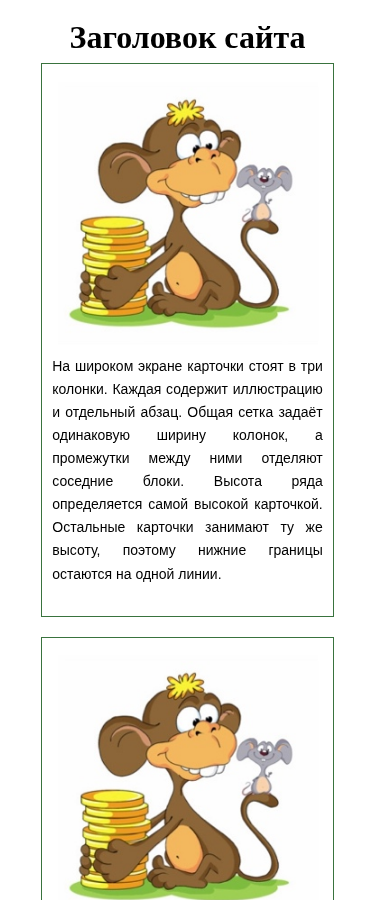
\includegraphics[width=\textwidth,height=125mm,keepaspectratio]{assets/mobile.png}
\caption{Верхняя часть страницы при ширине окна 375 px}
\end{figure}

\clearpage
\section{Результат}
Медиазапросы изменяют цвет текста и число колонок без JavaScript. Содержимое карточек и их порядок сохраняются при переходе между размерами окна. Высота карточек определяется содержимым, изображения загружаются локально.

\vspace{6mm}
\section*{Список использованных источников}
\begin{enumerate}[label=\arabic*.,leftmargin=8mm,itemsep=8pt,parsep=0pt]
\item Using media queries // MDN Web Docs. URL: \url{https://developer.mozilla.org/en-US/docs/Web/CSS/Guides/Media_queries/Using} (дата обращения: 20.10.2026).
\item Basic concepts of grid layout // MDN Web Docs. URL: \url{https://developer.mozilla.org/en-US/docs/Web/CSS/Guides/Grid_layout/Basic_concepts} (дата обращения: 20.10.2026).
\end{enumerate}

\clearpage
\section{Исходный код: index.html}
\listing{../index.html}

\clearpage
\section{Исходный код: style.css}
\listing{../style.css}

\clearpage
\section{Исходный код: media.html}
\listing{../media.html}

\vspace{8mm}
\section{Исходный код: media.css}
\listing{../media.css}
\end{document}
